\documentclass{beamer}

\mode<presentation>
{
  \usetheme{Berlin}
  \usecolortheme{default}
  \setbeamercovered{transparent}
}

\usepackage[english]{babel}
\usepackage[all]{xy}
\usepackage[latin1]{inputenc}

\usepackage{times}
\usepackage[T1]{fontenc}
\usepackage{verbatim}
\usepackage{hyperref}

\title[Sensor Fusion on a mini Unmanned Vehicle]
{Sensor Fusion on a mini Unmanned Vehicle}

\subtitle{Integrating vision-based algorithms on an Parrot AR.Drone to autonomously follow linear shaped structures in a landscape.}

\author[Verschoor ] % (optional, use only with lots of authors)
{C.~R.~Verschoor}

\institute[University of Amsterdam] % (optional, but mostly needed)
{
  Faculty of Science (FNWI) \\
  University of Amsterdam
}

\AtBeginSection[]
{
  \begin{frame}<beamer>{Outline}
    \tableofcontents[currentsection]
  \end{frame}
}

\begin{document}

\begin{frame}
  \titlepage
\end{frame}

\begin{frame}{Outline}
  \setcounter{tocdepth}{1}
  \tableofcontents
\end{frame}

\section{Introduction}
\subsection{Supervisors}
\begin{frame}{Supervisors}
\begin{center}
\begin{tabular}{ c c }
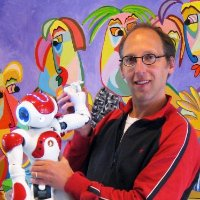
\includegraphics[width = 0.3\textwidth]{visser.jpg} & 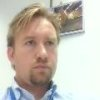
\includegraphics[width = 0.3\textwidth]{poppinga.jpg}\\
Dr. Arnoud Visser & Drs. Gerald Poppinga\\
Assistant Professor & R\&D Manager for mini UAS\\
University of Amsterdam & National Aerospace Lab NLR
\end{tabular}
\end{center}
\end{frame}

\begin{frame}{National Aerospace Lab NLR}
\begin{center}
\begin{tabular}{ c c }

\includegraphics[width = 0.3\textwidth]{nlr_logo.jpg} & 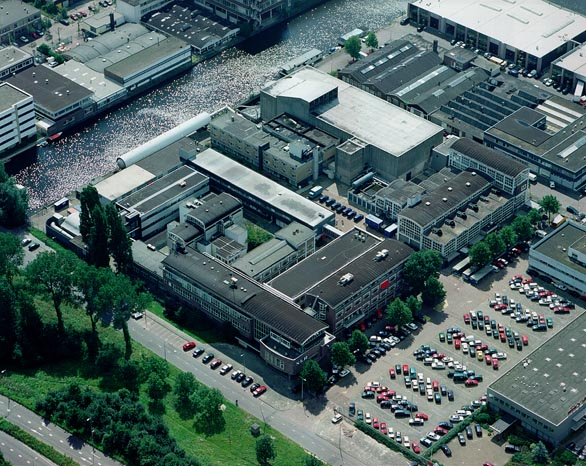
\includegraphics[width = 0.3\textwidth]{nlr_lucht.jpg}
\end{tabular}\\
NLR is the main knowledge enterprise in the Netherlands in the field of aviation and aerospace.
\end{center}
\end{frame}

\subsection{Research Question}
\begin{frame}
\begin{block}{Research Question}
What vision-based algorithms perform successful in autonomously following linear shaped structures in a landscape with an Parrot AR.Drone?
\end{block}
\begin{center}
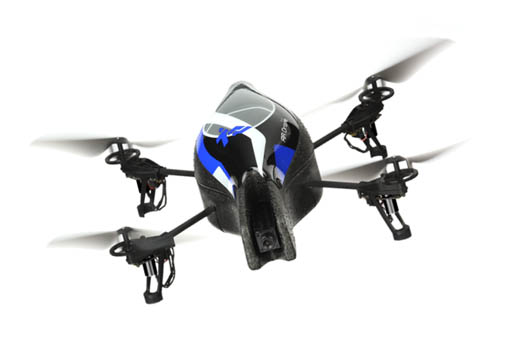
\includegraphics[width = 0.3\textwidth]{ardrone.jpg}
\end{center}
\end{frame}

\subsection{Research Goal}
\begin{frame}
\begin{block}{Research Goal}
The goal of this research project is to develop an algorithm on an Unmanned Aerial Vehichle that in the end can navigate autonomously over infrastructure.
\end{block}
\begin{center}
\begin{tabular}{ c c }
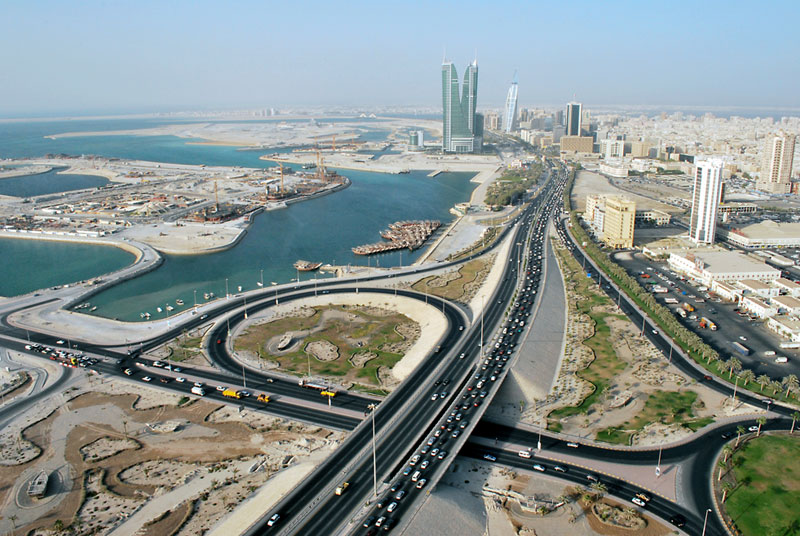
\includegraphics[width = 0.4\textwidth]{lucht_weg.jpg} & 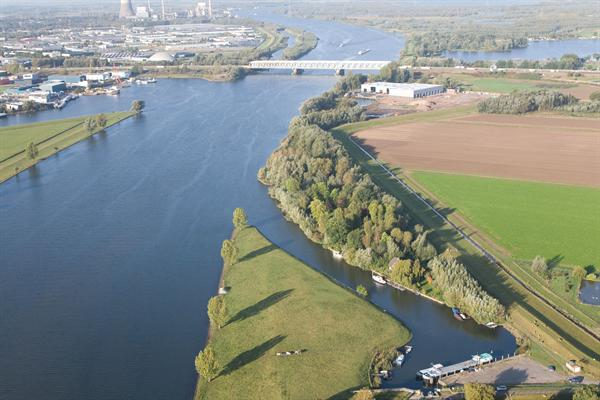
\includegraphics[width = 0.4\textwidth]{lucht_rivier.jpg}
\end{tabular}
\end{center}
\end{frame}

\begin{comment}
\subsection{Research Plan}
\begin{frame}{Research Plan in general}
\begin{enumerate}
\item Research relevant literature.
\item Define experiment tasks.
\item Create a dataset of the tasks.
\item Design vision-based algorithms.
\item Test vision-based algorithms in simulation experiments.
\item Test vision-based algorithms on the Asctec Pelican in experiments.
\item Based on the results either increase the difficulty of the task or improve the algorithms.
\item Compare algorithms.
\item Write research paper.
\end{enumerate}
\end{frame}

\begin{frame}{Experiment tasks}
Starting with an easily recognizable model and then gradually fade the preconditions away.\\
\textbf{Tasks:}
\begin{enumerate}
\item Follow a bright orange clothesline laying on the ground.
\item Follow a bright orange clothesline hanging in the air.
\item Follow a lighter orange clothesline hanging in the air.
\item Follow a white clothesline hanging in the air.
\end{enumerate}
\textbf{Extra tasks:}
\begin{enumerate}
\item Follow a white clothesline hanging in the air, while moving spirals around it.
\item Follow linear shaped structures in a landscape such as, highways, rivers and fences.
\end{enumerate}
\end{frame}

\subsection{Integration Plan}
\begin{frame}{Integration Plan}
\begin{enumerate}
\item Initial design.
\item Structural integration.
\item Algorithm and Data processing.
\item Intergrating software with the Flight Control System.
\item Interfacing with the Ground Control System.
\end{enumerate}
\end{frame}
\end{comment}

\section{Progress Overview}
\begin{frame}{Progress Overview}
\begin{itemize}
\item Platform change.
\item Set up the framework.
\item Overview Aproach
\item Implement vision-based algorithms.
\item Integrate vision-based algorithms.
\end{itemize}
\end{frame}

\subsection{Platform}
\begin{frame}{Platform change}
\textbf{Parrot AR.Drone} instead of \textbf{AscTec Pelican}.\\
\vspace{0.2cm}
\textbf{Reasons:}
\begin{itemize}
\item AR.Drone has integrated Optical Flow (hovering).
\item Framework is written for AR.Drone.
\item AscTec Pelican does not have Optical Flow integrated.
\end{itemize}
\textbf{Side effects:}
\begin{itemize}
\item AR.Drone carries a poorer camera.
\item AR.Drone does not carry pan/tilt camera.
\end{itemize}
\end{frame}

\subsection{Framework}
\begin{frame}{Setup the framework}
\begin{itemize}
\item Framework of MSc. student N. Dijkshoorn.\\
Provides:
\begin{itemize}
\item Real-time SLAM.
\item Communication AR.Drone.
\item Communication USAR-SIM Simulator.
\item Various controllers (ie. 3D mouse or keyboard).
\end{itemize}
\item Windows based.
\item Image library (OpenCV).
\item Source in C++.
\end{itemize}
\end{frame}

\subsection{Overview Approach}
\begin{frame}{Overview Line-Following Approach}
\xymatrix{Camera \ar[rr]_{stream} & & Framegrabber \ar[rr]_{frame} & & Line\ detection \ar[dd]_{\begin{bmatrix}x\\y\end{bmatrix}\ and\ \theta}\\
& & & &\\
World \ar[uu]_{input} & & Flight\ controller \ar[ll]_{flying} & & Navigation \ar[ll]_{controls}}
\end{frame}

\subsection{Vision-based algorithms}
\begin{frame}{Implementing vision-based algorithms}
\textbf{Line detection:}
Probabilistic/Randomized Hough Line  Transform
\begin{itemize}
\item Less computational costs due geometric features of a line.
\item Evaluates randomly selected points
\end{itemize}

\textbf{Line selection:} based on the features of the line (ie. length and slope).

\textbf{Determine movement:} Angle $\theta$ and transformation $\begin{bmatrix}x\\y\\\end{bmatrix}$

\textbf{Track line:} using area of interest.
\end{frame}

\begin{frame}{Video demonstration on dataset}
\href{http://youtu.be/GqdAJ3AUrmg}{Video: Probabilistic Hough Line Transform on Dataset Pelican}
\end{frame}

\subsection{Integration}
\begin{frame}{Integration of the vision-based algorithms}
\begin{itemize}
\item Link vision-based algorithm to the framework.
\item Determine action of the platform.
\end{itemize}

\textbf{Video:} AR.Drone following a line.
\end{frame}



\section{Planning}
\begin{frame}{Planning}
\begin{itemize}
\item Implement other vision-based algorithms.
\begin{itemize}
\item BioMAV's approach.
\item Majidi's approach
\end{itemize}
\item Improve flight actions of the line-following algorithm.
\item Compare algorithms.
\item Write Bachelor Thesis.
\end{itemize}
\end{frame}

\subsection{BioMAV's Approach}
\begin{frame}{BioMAV's Approach}

Combining:
\begin{itemize}
\item Enhanced Motion Detection Activation
\item Quick shift segmentation (Edge detection)
\end{itemize}
\end{frame}

\subsection{Majidi's Approach}
\begin{frame}{Majidi's Approach}
Combines
\begin{itemize}
\item Line Detection
\item Texture Segmentation
\end{itemize}
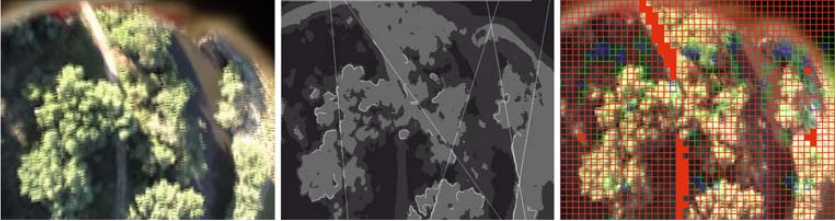
\includegraphics[width = \textwidth]{majidi.png}\footnote{\cite{Majidi2009}}
\end{frame}

\section{Questions}
\begin{frame}{Questions?}
\begin{center}
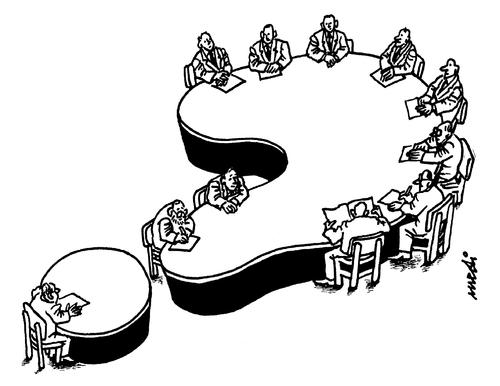
\includegraphics[width = 0.7\textwidth]{questions.jpg}
\end{center}
\end{frame}

\section{Relevant Literature}
\begin{frame}[allowframebreaks]{Relevant Literature}
\footnotesize
\nocite{*}
\bibliographystyle{apalike}
\bibliography{references}
\end{frame}

\end{document}
